\chapter{Einleitung}
\label{cha:Einleitung}


\section{Motivation}
Dieses Projekt findet im Rahmen der Vorlesung Systemnahe Programmierung an der Dualen Hochschule Baden-Württemberg statt. Ziel dieser Vorlesung ist es Kenntnisse über die systemnahe Programmierung zu vermitteln und so das Schreiben systemnaher Programme zu lernen. Innerhalb der Vorlesung wird Assembler für die 8051 Mikrokontroller verwendet. Um die erlernten Grundlagen dieser Vorlesung auch praktisch einsetzen zu können, wird ein Projekt erstellt und in einer virtuellen Entwicklungsumgebung ausgeführt. Dafür wurde die MCU-8051 IDE verwendet.  

Bei der Gestaltung des Projektes können die Studenten eigene Ideen umsetzen. Aufgrund unserer eigenen großen Sportleidenschaft haben wir uns dafür entschieden eine Fußballanzeigetafel mit Spielstand und Zeitanzeige zu implementieren. 


\section{Aufgabenstellung}
Die zu implementierende Anzeigetafel sollte sowohl den aktuellen Spielstand, sowie die bereits gespielte Zeit anzeigen (siehe Abb. \ref{fig:Anzeigetafel}). Dabei soll die Zahl der erzielten Tore oder Punkte über angeschlossene  Knöpfe steuerbar sein. Optional zu diesen Implementierungen soll zusätzlich eine Hupe die bei Ablauf der Spielzeit ertönt implementiert werden. Der aktuelle Spielstand und die Zeit soll per Knopfdruck zurück setzbar sein. 

Für die Implementierung der Anzeigetafel werden nur die innerhalb der Entwicklungsumgebung vorgegebenen Hilfsmittel genutzt. 

\begin{figure}[h]
	\centering
	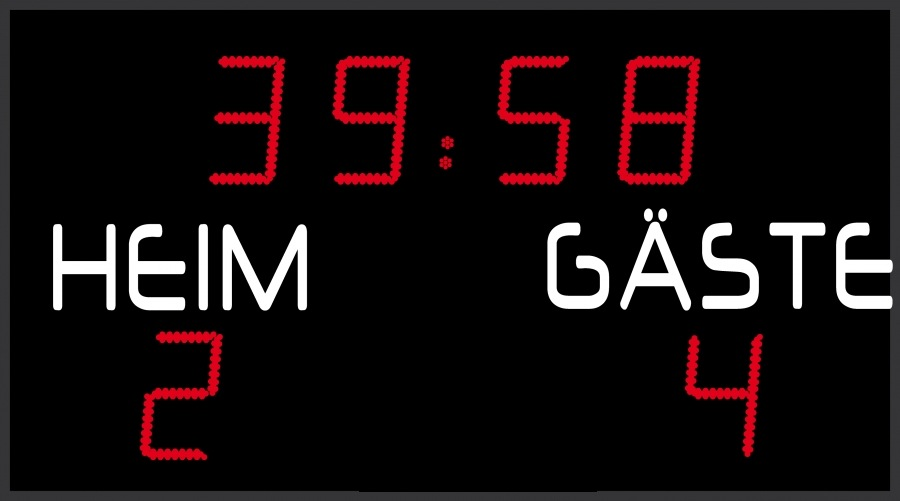
\includegraphics[width=0.9\textwidth]{Anzeigetafel} 
	\caption{Abbildung Anzeigetafel  https://pimage.sport-thieme.de/detail-fillscale-min-height/stramatel-anzeigetafel-ffbffc/131-5400 }
	\label{fig:Anzeigetafel}
\end{figure}